%%%%%%%%%%%%%%%%%%%%%%%%%%%%%%%%%%%%%%%%%%%%%%%%%%%%%%%%%%%%%%%%%%%%%%%%%%%%%
% chapters/chapter-2.tex
%%%%%%%%%%%%%%%%%%%%%%%%%%%%%%%%%%%%%%%%%%%%%%%%%%%%%%%%%%%%%%%%%%%%%%%%%%%%%

\chapter{Main results}
\label{chap:main}

\begin{figure}[H]
  \centering{}\begin{tikzpicture}[x=1mm,y=1mm,scale=\textwidth/140mm]
  \node[anchor=south west, inner sep=0] at (0,4) {
    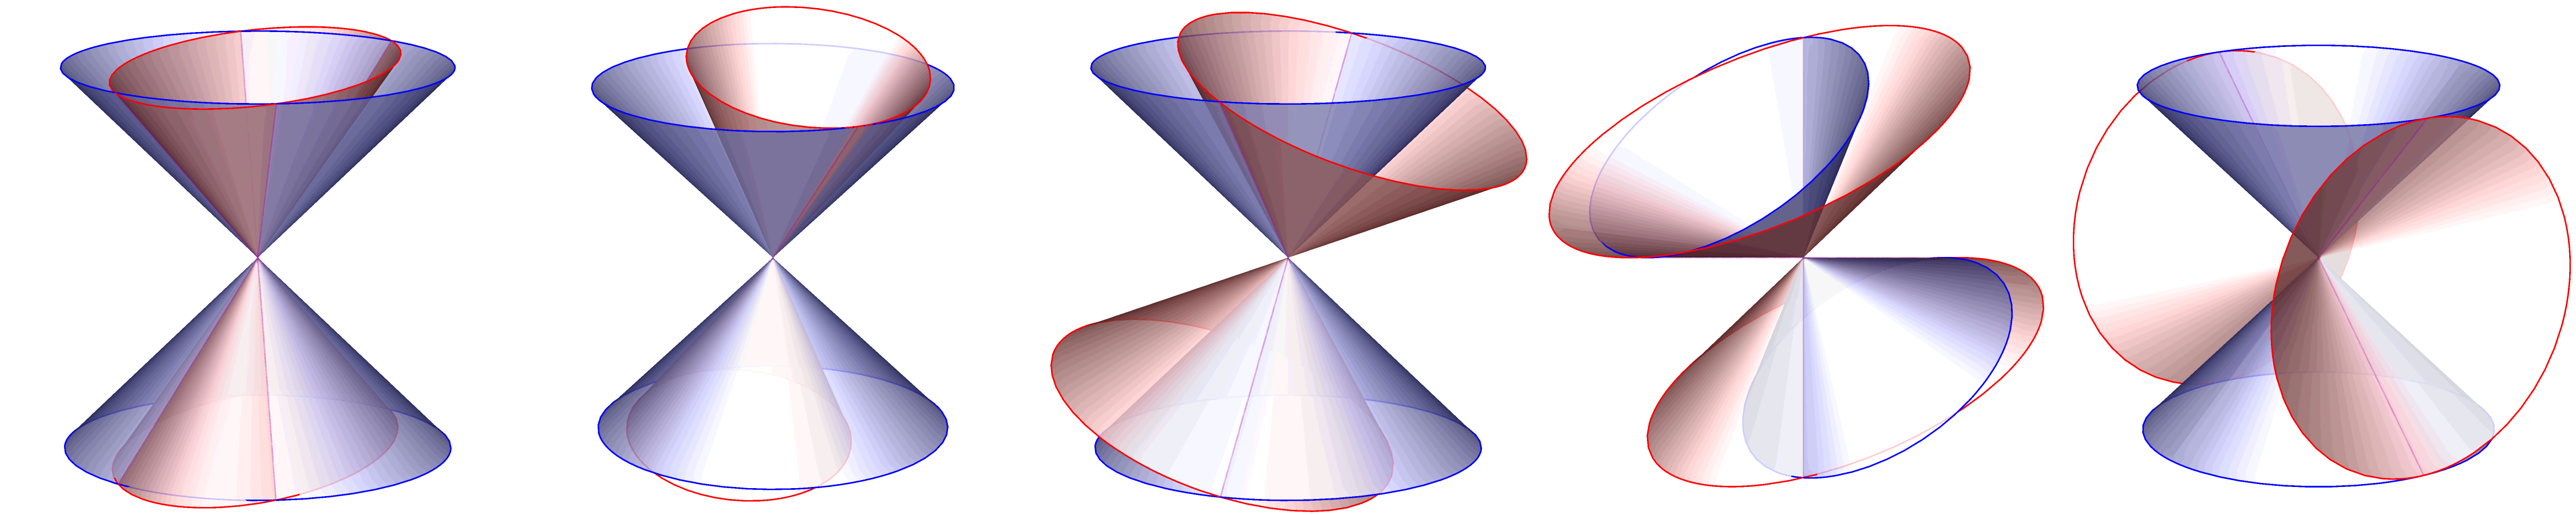
\includegraphics[width=\textwidth]{figures/test-figure}
  };
  \node[] at (0*28+14,0) {Type I};
  \node[] at (1*28+14,0) {Type IIa};
  \node[] at (2*28+14,0) {Type IIb};
  \node[] at (3*28+14,0) {Type III};
  \node[] at (4*28+14,0) {Type IV};
  \end{tikzpicture}\vspace{-0.6ex}
  
  \caption{\label{fig:classification}Allowed null cone configurations.}
\end{figure}

\begin{table}[H]
  \caption{\label{tab:classification}Allowed local metric configurations.}
  \vspace{-1ex}
  
  \noindent\centering{}\hspace{-3mm}
  \bgroup\renewcommand{\arraystretch}{1.5}
  \begin{tabular}{cccc} \hline\hline
    Type % & Segre char. 
    & $\diag(g)$ & $\diag(f)$ & $\diag(g^{-1}f)$ 
    \\ \hline
    \textbf{I} % & $[1111]$ 
    & $(-1,1,1,1)$ 
    & $(-\lambda_1,\lambda_2,\lambda_3,\lambda_4)$
    & $(\lambda_1,\lambda_2,\lambda_3,\lambda_4)$
    \\
    \textbf{IIa} % & $[211]$ 
    & $(\pm\!
    \begin{pmatrixc} 0&1\\[-0.2em]1&0\end{pmatrixc}\!,1,1 )$
    & $(\pm\!
    \begin{pmatrixc} 0&\lambda\\[-0.2em]\lambda & 1 \end{pmatrixc}\!,
    \lambda_2,\lambda_3)$
    & $(\begin{pmatrixc} \lambda&1\\[-0.2em]0 & \lambda \end{pmatrixc}\!,
    \lambda_2,\lambda_3)$
    \\[0.8em]
    \textbf{IIb} % & $[z\bar{z}11]$ 
    & $(\pm\!
    \begin{pmatrixc} 0 & 1 \\[-0.2em]1 & 0 \end{pmatrixc}\!,1,1)$ 
    & $(\pm\!
    \begin{pmatrixr}b & a \\[-0.2em] a & -b \end{pmatrixr}\!,
    \lambda_2,\lambda_3)$ 
    & $(
    \begin{pmatrixr}a & -b \\[-0.2em] b & a \end{pmatrixr}\!,
    \lambda_2,\lambda_3)$ 
    \\[0.8em]
    \textbf{III} % & $[31]$ 
    & $(\begin{pmatrixc} 0&0&1\\[-0.2em]
    0 & 1 & 0\\[-0.2em]
    1 & 0 & 0 \end{pmatrixc}\!,1)$
    & $(\begin{pmatrixc} 0&0&\lambda\\[-0.2em]
    0 & \lambda &1\\[-0.2em]
    \lambda & 1 & 0 \end{pmatrixc}\!,\lambda_2)$
    & $(\begin{pmatrixc} \lambda&1&0\\[-0.2em]
    0 & \lambda &1\\[-0.2em]
    0 & 0 & \lambda \end{pmatrixc}\!,\lambda_2)$
    \\
    \textbf{IV} % & $[(11)11]$ 
    & $(-1,1,1,1)$ 
    & $(\lambda,-\lambda,\lambda_2,\lambda_3)$
    & $(-\lambda,-\lambda,\lambda_2,\lambda_3)$
    \\ \hline\hline
  \end{tabular}
  \egroup
\end{table}